%%%INTRODUCCIÓN GENERAL%%%
\chapter{Introducción}
\section{Nanociencia}
El prefijo nano deriva del griego \emph{nanos}, que significa literalmente ``enano''. En el sistema internacional de unidades, el prefijo nano representa un factor de $\mathrm{10^{-9}}$, o una mil millonésima parte. Al añadir este prefijo a la unidad de longitud, obtenemos ``nanómetro'' (nm), o una mil millonésima parte de un metro. Así la nanotecnología es, a grandes rasgos, la ciencia, tecnología, e ingeniería que trata sistemas en el rango aproximado de 1-100 nanómetros \citep{Haick2013,Gressler2013}. Esta definición es práctica pero resulta poco precisa, un nanomaterial debe ser considerado como tal cuando comienza a exhibir un cambio en sus propiedades debido a la reducción de sus dimensiones, ésta es propia de cada material y por tanto no puede ser estandarizada. Se ha de tener claro en qué rango de dimensiones se encuentra la escala nanométrica, los seres humanos estamos acostumbrados a escalas grandes, se nos hace fácil entender las comparaciones de kilómetros con metros, o milímetros con metros, pero al reducir el tamaño a micrómetros o nanómetros nos cuesta, pues son escalas que se escapan de nuestros sentidos. Para ponerlo en perspectiva, un nanómetro es a un metro, como un metro es a un millón de kilómetros. La figura \ref{fig:scale} muestra una escala de tamaños con varios ejemplos desde la escala humana hasta la atómica.

\begin{figure}[h!]
	\centering
	\fbox{
		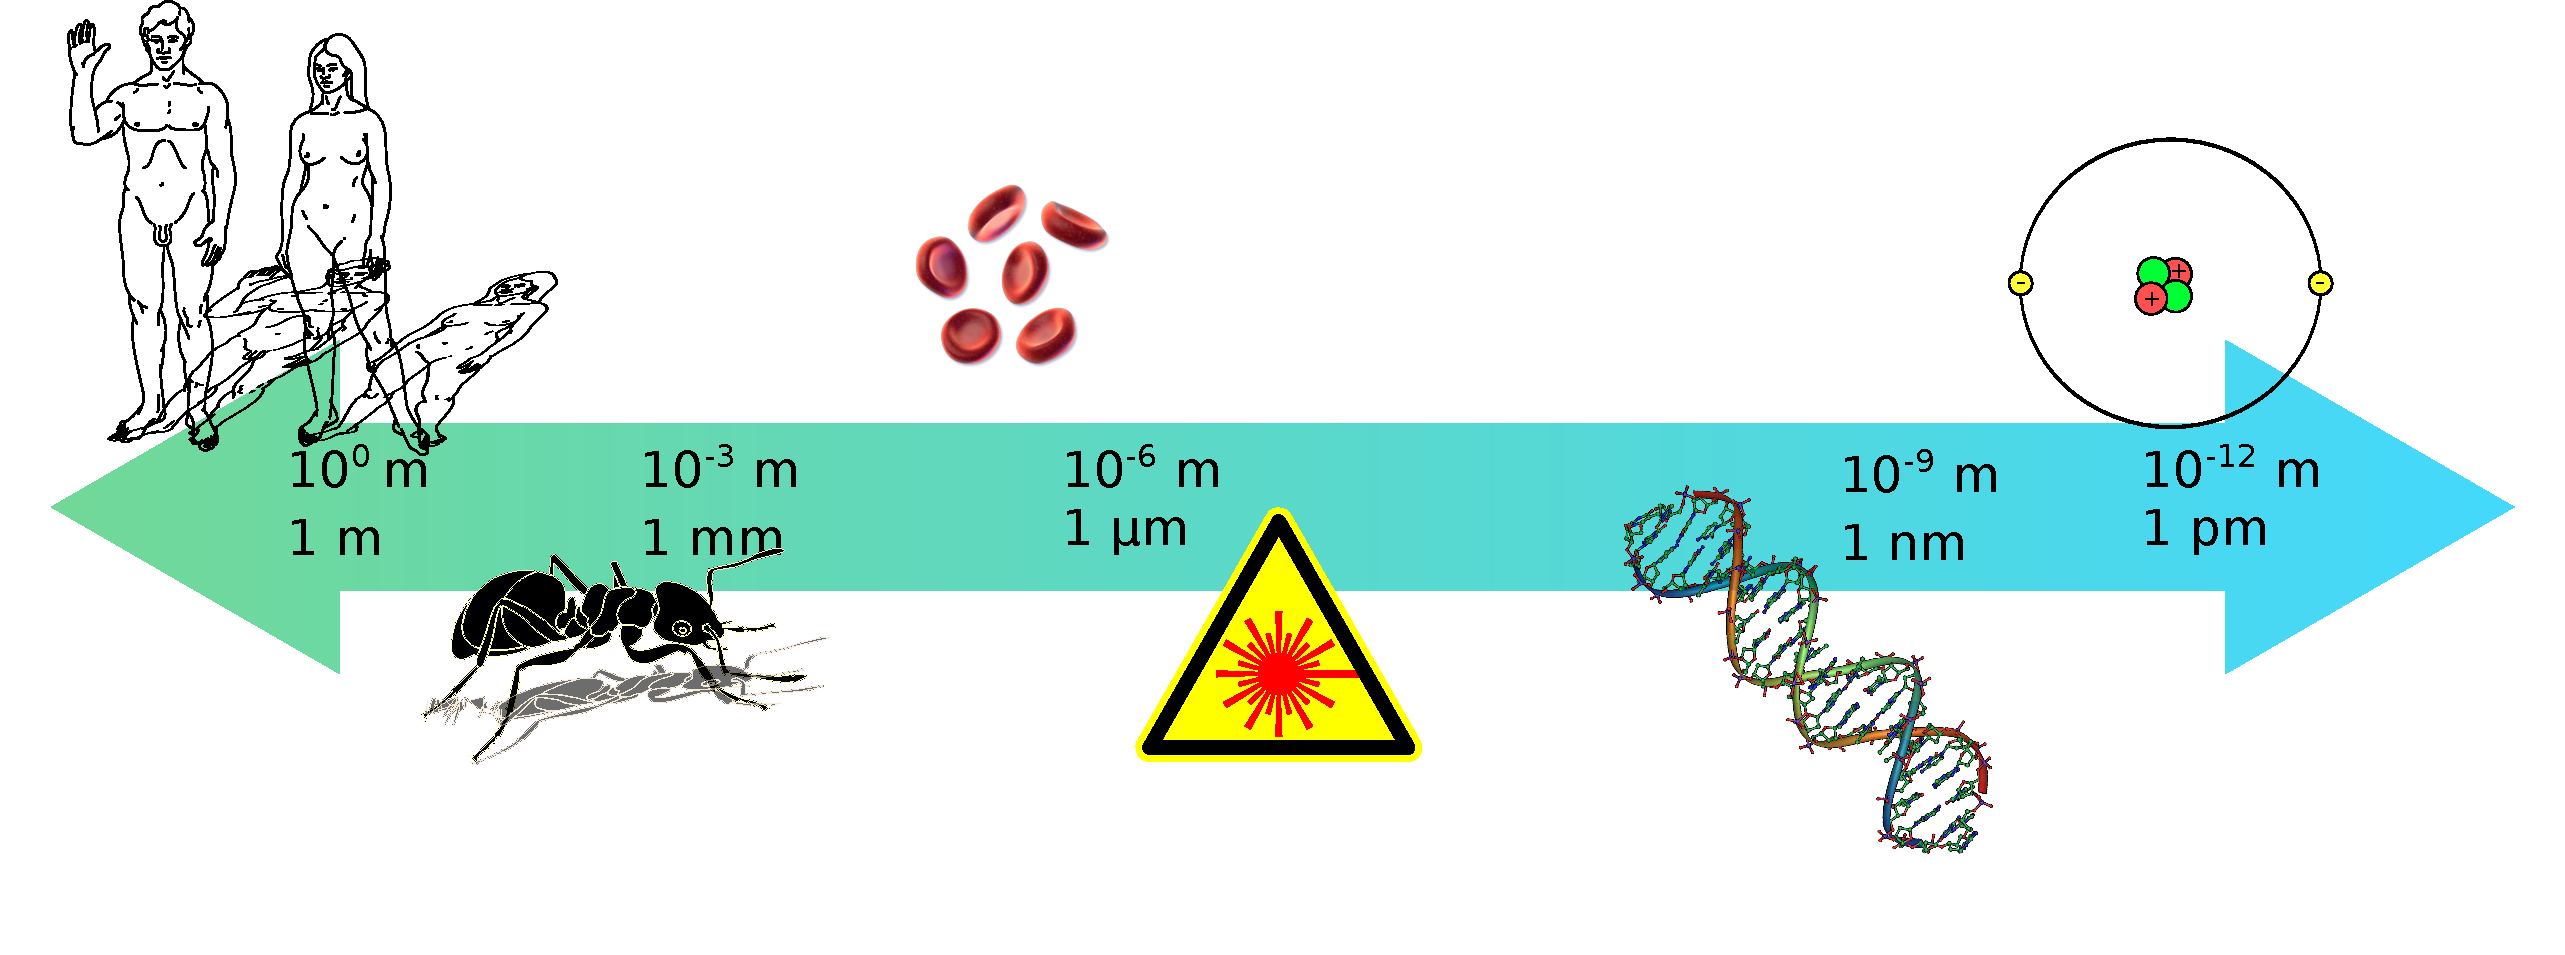
\includegraphics[width=\textwidth]{scale.pdf}
	}
	\caption[Comparativa de ódenes de magnitud desde metros hasta picometros]{Comparativa de órdenes de magnitud. De izquierda a derecha: Escala humana 1-2 m. Insectos 10 cm - 1 mm. Glóbulos rojos 6 $\mathrm{\mu}$m. Longitud de onda de luz visible 780-380 nm. Doble hélice de ADN 2 nm. Radio atómico de un átomo de helio 31 pm.}
\label{fig:scale}
\end{figure}

La idea de la nanotecnología fue vislumbrada, entre otros, por el físico Richard Feynman y expuesta en su charla \emph{``There is plenty room at the bottom''} \citep{Feynman1960}. Feynman plantea que no existen barreras físicas que impidan manipular sistemas nanométricos, moléculas, o incluso átomos. La era moderna de la nanotecnología comienza con el desarrollo del microscopio de efecto túnel por Binning y Rohrer en 1981 \citep{Binnig1982}, que les hizo ganar el Premio Nobel de Física en el año 1986. Un microscopio de efecto túnel (STM por sus siglas en inglés \emph{Scanning Tunneling Microscope}), puede superar resoluciones de 0,1 nm de resolución lateral, 0,01 nm en profundidad, y trabajar en variadas condiciones, sin necesidad de alto vacío o bajas temperaturas. Además de poder resolver átomos, el STM también puede manipularlos \citep{Chen2008}.

Una forma simple de clasificar los nanomateriales surge del número de dimensiones del material que no están en la nanoescala (ver figura \ref{fig:carbon_allotropes}). Un material que no posee ninguna dimensión en la nanoescala (material \emph{bulk}), se denomina material 3D y no  se considera un nanomaterial\footnote{A veces se les llama nanomateriales 3D a materiales formados por nanomateriales (2D, 1D, o 0D), que forman estructuras tridimensionales macroscópicas y muestran propiedades de nanomateriales, como por ejemplo, los aerogeles.}. Si una dimensión del material está en la nanoescala, se habla de material 2D, análogamente, con dos dimensiones en la nanoescala se trata de un nanomaterial 1D, y por último, si todas las dimensiones están en la nanoescala se denomina nanomaterial 0D.

\begin{figure}
	\centering
	\begin{subfigure}[b]{0.2\textwidth}
		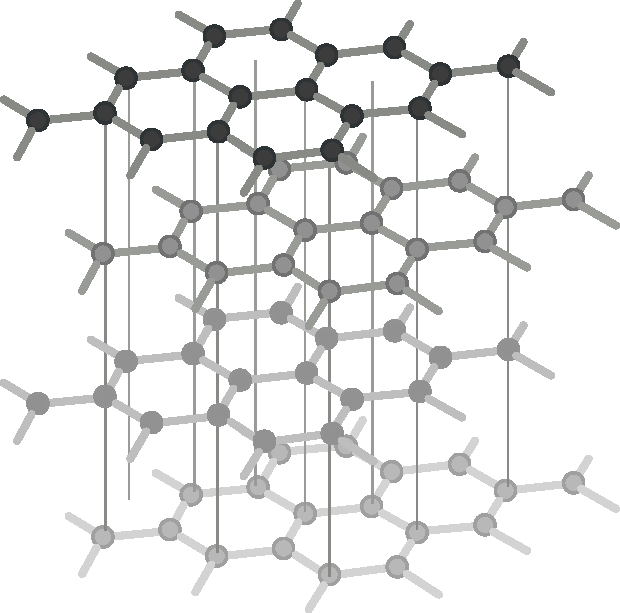
\includegraphics[width=\textwidth]{graphite_structure.pdf}
		\caption{}
		\label{fig:graphite_struct}
	\end{subfigure}
	\begin{subfigure}[b]{0.2\textwidth}
		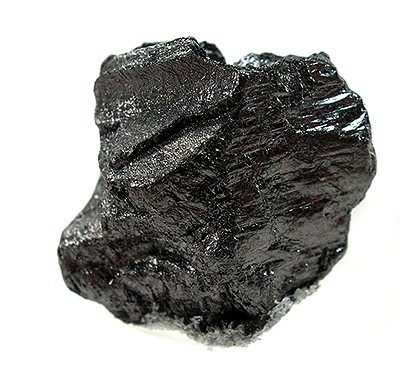
\includegraphics[width=\textwidth]{graphite_image.jpg}
		\caption{}
		\label{fig:graphite_image}
	\end{subfigure}
	\begin{subfigure}[b]{0.2\textwidth}
		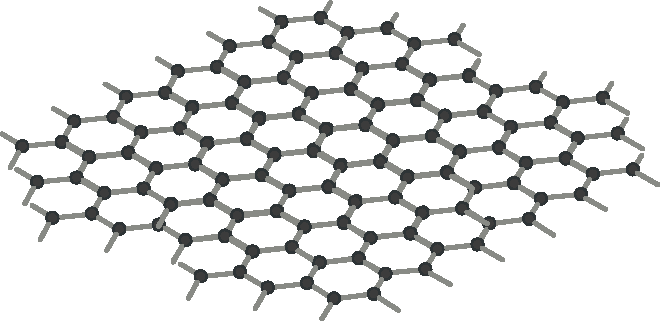
\includegraphics[width=\textwidth]{graphene_structure.pdf}
		\caption{}
		\label{fig:graphene_struct}
	\end{subfigure}
	\begin{subfigure}[b]{0.2\textwidth}
		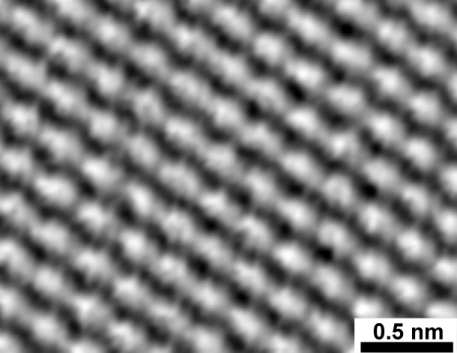
\includegraphics[width=\textwidth]{graphene_image.jpg}
		\caption{}
		\label{fig:graphene_image}
	\end{subfigure}
\\
	\begin{subfigure}[b]{0.2\textwidth}
		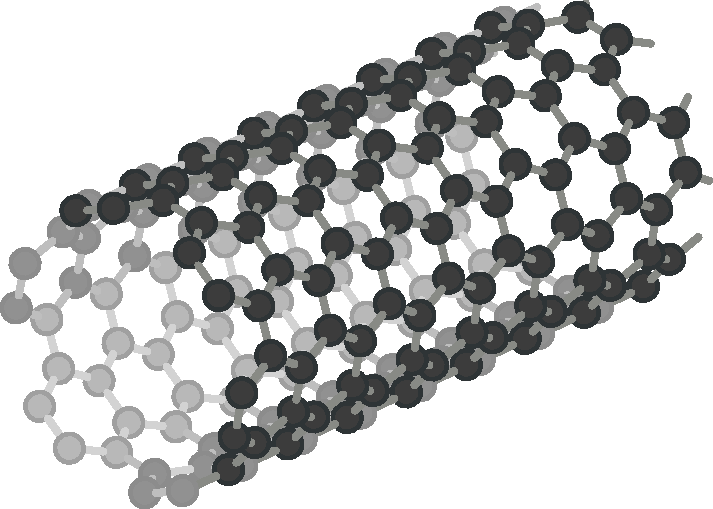
\includegraphics[width=\textwidth]{cnt_structure.pdf}
		\caption{}
		\label{fig:cnt_struct}
	\end{subfigure}
	\begin{subfigure}[b]{0.2\textwidth}
		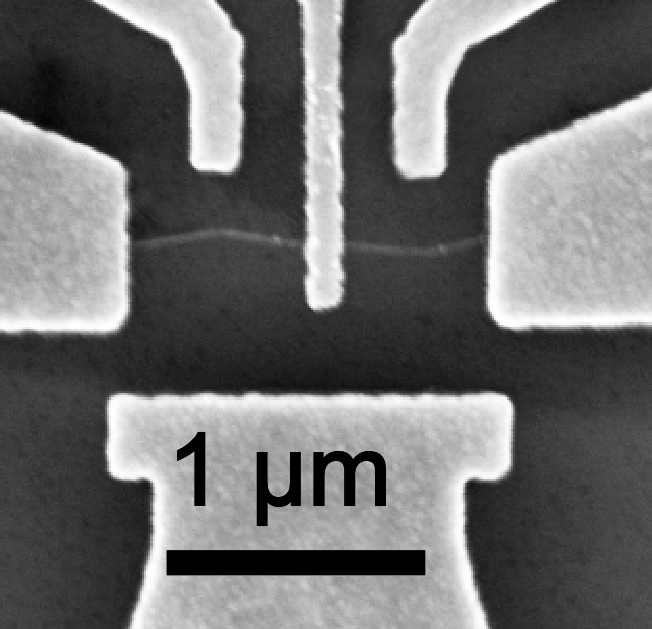
\includegraphics[width=\textwidth]{cnt_image.png}
		\caption{}
		\label{fig:cnt_image}
	\end{subfigure}
	\begin{subfigure}[b]{0.2\textwidth}
		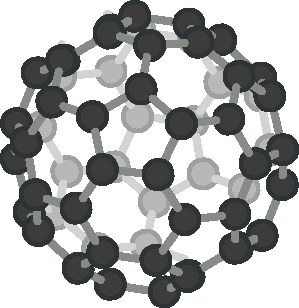
\includegraphics[width=\textwidth]{fullerene_structure.pdf}
		\caption{}
		\label{fig:fullerene_structure}
	\end{subfigure}
	\begin{subfigure}[b]{0.2\textwidth}
		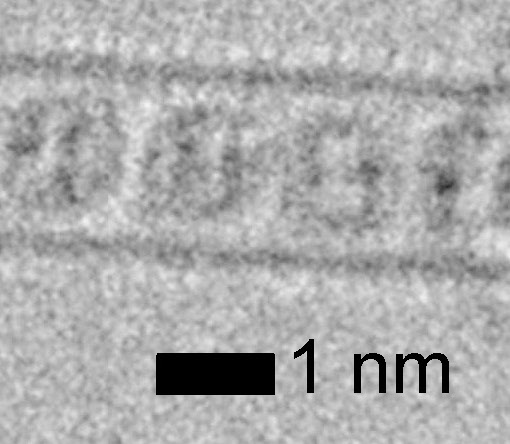
\includegraphics[width=\textwidth]{fullerene_image.jpg}
		\caption{}
		\label{fig:fullerene_image}
	\end{subfigure}
	\caption[Alótropos del carbono mostrando las diferentes dimensionalidades de los nanomateriales]{Estructuras e imágenes de varios alótropos del carbono como ejemplos de la dimensionalidad de los nanomateriales:  \subref{fig:graphite_struct} y \subref{fig:graphite_image} grafito natural, un material 3D. \subref{fig:graphene_struct} y \subref{fig:graphene_image} grafeno, imagen de microscopia de efecto túnel (Frank Trixler, LMU/CeNS: Organic Semiconductor Group), un material 2D. \subref{fig:cnt_struct} y \subref{fig:cnt_image} nanotubo de carbono, imagen SEM de un dispositivo para medir diferentes propiedades del nanotubo (Pavlos Apostolidis, London Centre for Nanotechnology, Department of Physics \& Astronomy), un material 1D. \subref{fig:fullerene_structure} y \subref{fig:fullerene_image} fullereno, imagen TEM de fullerenos C80 funcionalizados dentro de un nanotubo de carbono \citep{Gimenez2011}, un material 0D.}
	\label{fig:carbon_allotropes}
\end{figure}

\subsection{La física de sistemas nanométricos}
Al reducir las dimensiones a escalas nanométricas, surgen efectos de confinamiento cuántico, pues se restringe el movimiento de los electrones en el material, esto conlleva a la discretización de los niveles de energía de los electrones y al cambio de la densidad de estados del material al tratarse de semiconductores (figura \ref{fig:DoE}). Dependiendo de cuantas dimensiones son llevadas a la nanoescala, es como se ve afectada la densidad de estados.

\begin{figure}[h!]
	\centering
	\fbox{
		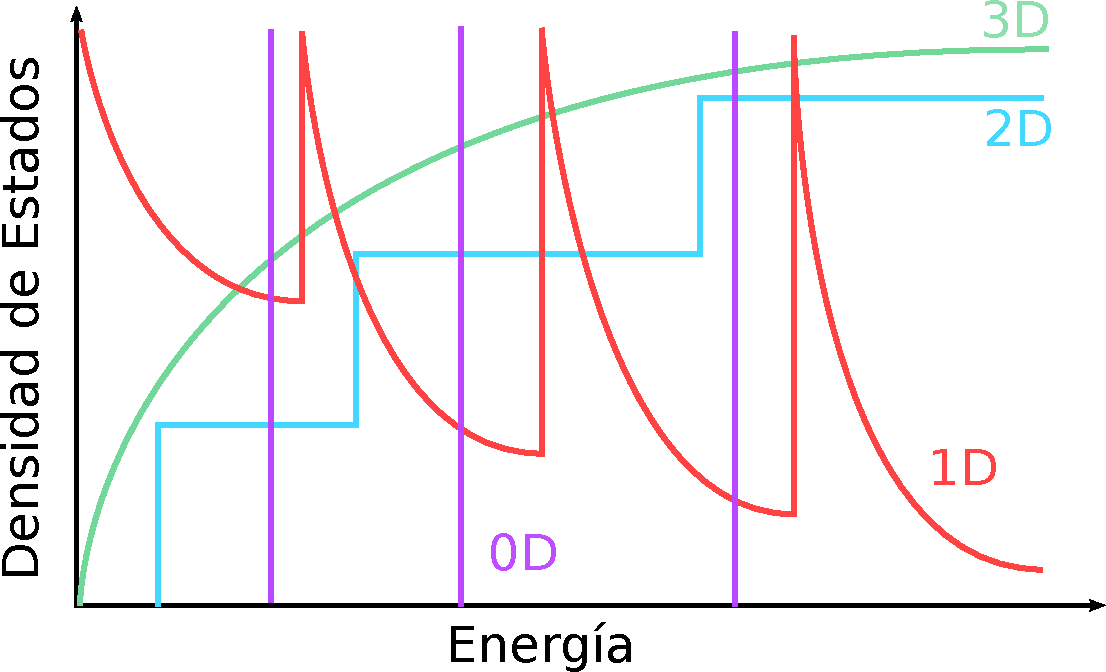
\includegraphics[width=0.6\textwidth]{DoE.pdf}
	}
	\caption[Densidad de estados en diferentes dimensionalidades]{Densidad de estados diferentes dimensiones. Para materiales 3D (no nanoestructurados), la densidad de estados es continua. En nanomateriales 2D, la densidad de estado forma escalones. Para materiales 1D, ésta es discontinua, y para nanomateriales 0D es completamente discreta. }
	\label{fig:DoE}
\end{figure}

Por otra parte, si un determinado volumen es dividido en partículas más pequeñas, el área superficial aumenta. Por ejemplo, como se muestra en la secuencia de la figura \ref{fig:area_cubes}, el volumen total, o cantidad de material en cada división no cambia, pero el área superficial se duplica \footnotemark, siguiendo está lógica, al fragmentar un cubo de lado 1 cm a cubos de lado 100 nm, el área total habrá aumentado 100.000 veces. El aumento del área superficial aumenta la reactividad del material, ya que hay más lugar para reacciones químicas. Otra forma de verlo, es considerar la proporción de átomos en la superficie, con la cantidad de átomos al interior de una partícula, en la figura \ref{fig:graph_nanocube} se muestra como aumenta esta proporción al disminuir el tamaño de una nanopartícula.

\footnotetext{Si en la secuencia de la figura \ref{fig:area_cubes} el cubo más grande tiene lado $l$, su área superficial es $6 \times l^2$, en la primera división, el lado de cada cubo es $l/2$ y el área de cada uno es $6\left( l/2\right)^2$, que en total hacen $6\left(l/2\right)^2\times 8$, en la segunda división el área total es $6\left(l/4\right)^2\times 8 \times 8$, así, en la n-ésima división el área es $6l^2 \left(1/2^n\right)^2\times 8^n$ o $6l^2 \times 2^n$. Así, el área superficial se dobla con cada división.}

\begin{figure}[h!]
	\centering
	\begin{subfigure}{\textwidth}
		\fbox{
			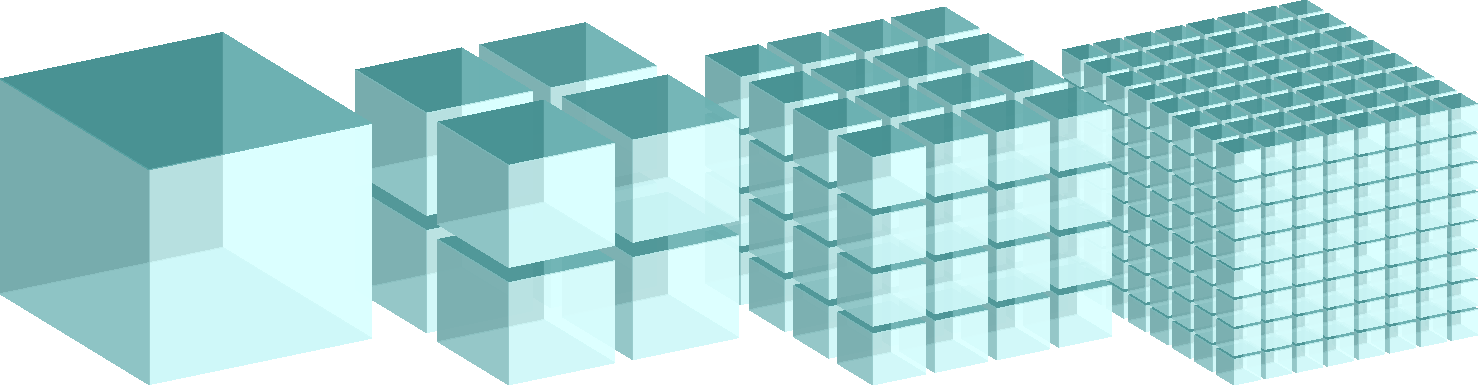
\includegraphics[width=\textwidth]{area_cubes.pdf}
			}
		\caption[Subdivisiones de un cubo demostrando el aumento de área superficial total]{Subdivisiones de un cubo demostrando el aumento de área superficial total.}
		\label{fig:area_cubes}
	\end{subfigure}
	\begin{subfigure}{\textwidth}
			\begin{tikzpicture}[]
				\begin{axis}[
				width=\textwidth,
				height=\axisdefaultheight,
				change x base,
				cycle list name=colorbrewer-RYB,
				width = \textwidth,
				ylabel={Proporción de átomos},
				yticklabel=\pgfmathparse{100*\tick}\pgfmathprintnumber{\pgfmathresult}\,\%,
				xlabel={Tamaño de partícula},
				x unit=m,
				x SI prefix=nano,
				legend entries={En la superficie, Dentro de la partícula}]	
				\addplot table [x expr = \thisrow{l}, y expr=\thisrow{surf}] {./Data/nanocube.txt};
				\addplot table [x expr = \thisrow{l}, y expr=\thisrow{bulk}] {./Data/nanocube.txt};
				\end{axis}
			\end{tikzpicture}
			\caption{Proporción de átomos en la superficie y dentro de cada nanopartícula en relación a su tamaño.}
			\label{fig:graph_nanocube}
	\end{subfigure}
	\caption[Aumento de área superficial y proporcion de átomos en superficie al disminuir el tamaño de las nanopartículas]{\subref{fig:area_cubes}Si se subdivide un cubo de 1 cm de lado hasta tener cubos de 100 nm de lado, el área superficial total pasaría de 6 $\mathrm{cm^2}$ a 60 $\mathrm{m^2}$. En este caso, el lado de cada cubo disminuye 100.000 veces, aumentando el área superficial total por el mismo factor. \subref{fig:graph_nanocube} surface energy.}
\end{figure}

\subsection{Síntesis de nanomateriales}
Dependiendo de la vía de aproximación a la nanoescala, se distinguen dos formas de síntesis, por un lado, si partimos de la forma macroscópica de un material y de algún modo se reducen sus dimensiones hacia la nanoescala, se habla de un proceso \textit{top-down}, por ejemplo la exfoliación del grafito (\textit{bulk material}) para obtener grafeno (nanomaterial) \citep{Novoselov2004}.  Por otro lado, sintetizar un nanomaterial a partir de átomos o moléculas es un proceso \textit{bottom-up}, un ejemplo es la síntesis de nanopartículas de oro a partir de un precursor como el ácido tetracloroaúrico \citep{Daniel2004}.

\subsection{Caracterización de nanomateriales}
Los nanomateriales son caracterizados usando técnicas comunes que se utilizarían para materiales no nanoestructurados dependiendo de las características que se deseen estudiar.
